\section{Introducción}

\hspace{1mm} En este trabajo practico, se busca comprender, diseñar e implementar un amplificador clase A en RF. Debido a que en RF, las longitudes de onda son del orden de los componentes que se utilizan típicamente, como resistencias, capacitores, etc. lo que imposibilita la utilización de los parámetros concentrados. Por lo tanto, se utiliza el concepto de parámetros distribuidos para diseñar el circuito mediante microtiras.

\section{Marco teórico}
\hspace{1mm} Los parámetros distribuidos se utilizan en RF para modelar y comprender el comportamiento de las señales a lo largo de las lineas de transmisión. La tensión y corriente comienzan a depender de la posición y del tiempo. %revisar
Esto hace que estos sean complejos de medir, debido a que según la posición en donde se coloque el instrumento de medición, la medición seria distinta. Uno de los modelos de parámetros concentrados mas utilizados son los Z, donde estos representan las impedancias de una determinada red. Para poder calcular los parámetros Z se debe realizar un cortocircuito o circuito abierto según corresponda, ya sea en la entrada o la salida. Realizar esto en alta frecuencia es complicado, por lo que no resulta una opción utilizar parámetros concentrados.
Es por esto que se utilizan  RF se utilizan los parámetros distribuidos, para modelar y comprender el comportamiento de las señales a lo largo de las lineas de transmisión,
Un circuito resonante LC está compuesto por un inductor L y un capacitor CT, estos se conectan como se observa en la figura 1.

\begin{figure}[!h]
    \centering
    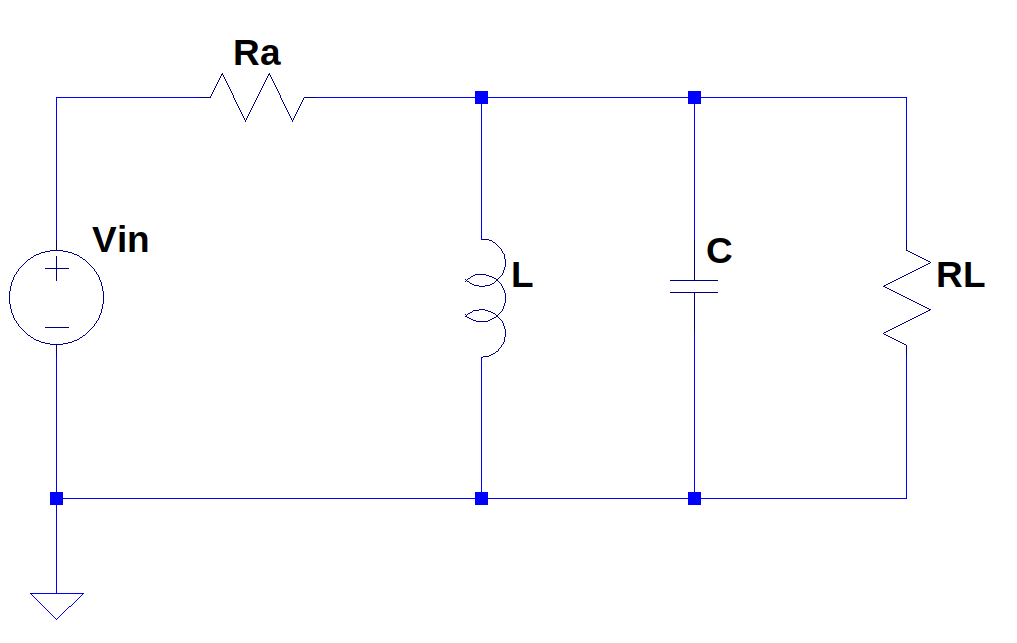
\includegraphics[width=0.8\textwidth]{Imagenes/LC.png}
    \caption{Circuito LC}
    \label{fig:LC}
\end{figure}

\hspace{1mm} Este circuito va a tener una frecuencia de resonancia donde la misma se encuentra mediante la siguiente ecuación:

\begin{equation}
    f_o = \frac{1}{2\pi \sqrt{LC}}
\end{equation}

\hspace{1mm} Por lo tanto, hay múltiples combinaciones de \(L\) y \(C\) para una determinada frecuencia de resonancia.
Otro parámetro importante en estos circuitos, es el factor de calidad \(Q\), para este circuito se analizan dos factores de calidad. Por un lado, el factor de calidad cargado \( Q_{\text{c}} \) el cual tiene sentido cuando la carga está conectada al circuito resonante, mientras que el descargado \( Q_{\text{d}} \) cuando el circuito no tiene carga. Las ecuaciones de estos parámetros son las siguientes:

\begin{equation}
    Q_d = \frac{R_p}{X_L} 
\end{equation}

\begin{equation}
    Q_c = \frac{fo}{BW} = \frac{R_T}{X_L}
\end{equation}

%Siendo:
%\begin{equation}
%   R_T = R_a//R_p//R_L
%\end{equation}
\newpage
Donde:
\begin{itemize}
    \item \( f_o \) es la frecuencia de resonancia,
    \item \( BW \) es el ancho de banda del circuito,
    \item \( R_T \) es la resistencia total del circuito,
    \item \( R_a \) es la resistencia del generador,
    \item \( R_p \) es la resistencia parásita del inductor
    \item \( R_L \) es la resistencia de carga del circuito, y
    \item \( X_L \) es la reactancia inductiva. 
    
\end{itemize}

Es evidente, que si se tiene una frecuencia de resonancia dada y deseáramos definir el ancho de banda, el valor de las resistencias que componen a \( R_T \), tanto \( R_a \) como  \( R_L \) no se podrían modificar debido a que son valores fijos y \( R_p \) depende del diseño de la bobina. Por lo tanto, se plantea una forma de solucionar dicho inconveniente, modificando el hecho de tener un solo capacitor total \(C_T\), a tener 4 capacitores que en conjunto sigan siendo equivalentes a \(C_T\), lo que resulta en que \( f_o \) no se modifica. Lo siguiente es que la entrada como la salida se conecten al punto medio para con esto, poder plantear un modelo equivalente mucho mas sencillo de analizar al reflejar \( R_a \) y \( R_L \) y de esta forma todas las resistencias queden en paralelo a \( R_p \).

\begin{figure}[!h]
    \centering
    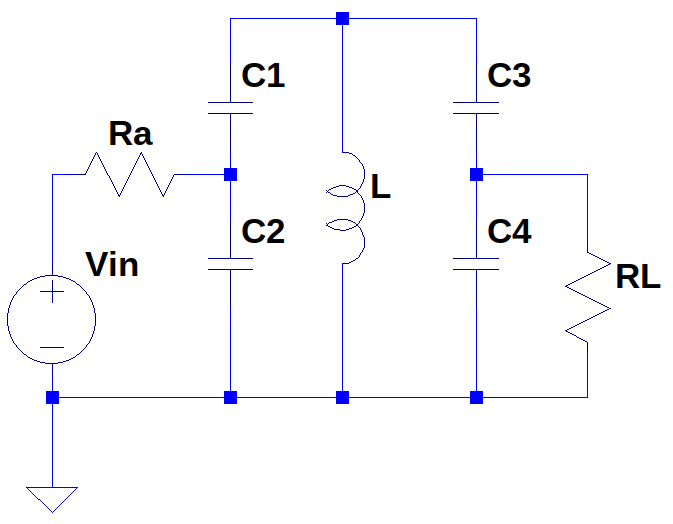
\includegraphics[width=0.8\textwidth]{Imagenes/LC_2.png}
    \caption{Circuito LC con 4 capacitores}
    \label{fig:LC_2}
\end{figure}

Para que \( f_o \) se mantenga en el mismo valor, los capacitores deben cumplir la siguiente ecuación:  

\begin{equation}
    \frac{C_T}{2} = \frac{C_1C_2}{C_1+C_2} = \frac{C_3C_4}{C_3+C_4}
\end{equation}
Luego, para reflejar las resistencias, se utiliza el concepto de un autotransformador:
\begin{figure}[!h]
    \centering
    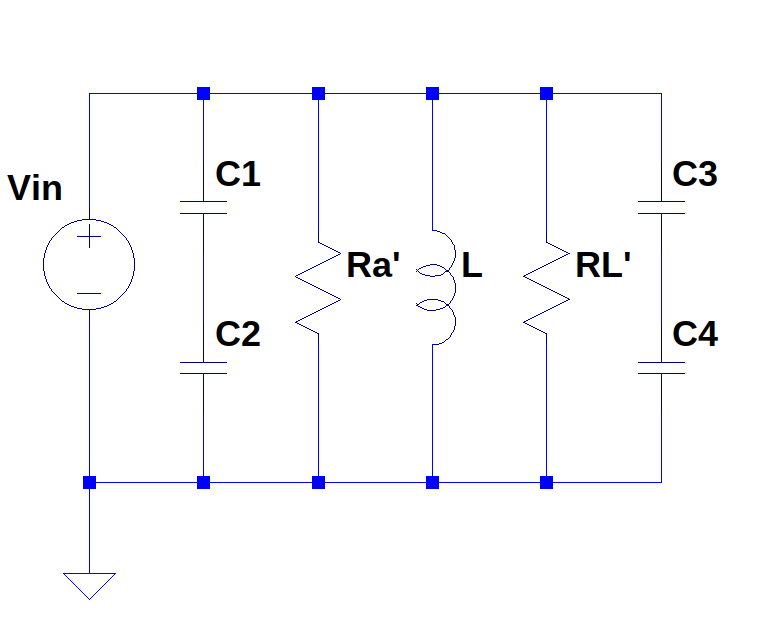
\includegraphics[width=0.8\textwidth]{Imagenes/LC_3.png}
    \caption{Circuito LC reflejado}
    \label{fig:LC_3}
\end{figure}
\begin{equation}
    R_a' = (1+\frac{C_2}{C_1})^2R_a
\end{equation}

\begin{equation}
    R_L' = (1+\frac{C_4}{C_3})^2R_L
\end{equation}

Por lo tanto,
\begin{equation}
    R_T = R_a'//R_p//R_L' 
\end{equation}

Finalmente, se deben cumplir las siguientes ecuaciones:

\begin{equation}
    2R_T = (R_L'//R_p) 
\end{equation}

\begin{equation}
    2R_T = R_a' 
\end{equation}

Para que de esta forma, el paralelo de la ecuación (8) y (9) resulten en \(R_T\) 
\newpage
\subsection{Redes L}
Esta se trata de uno de los acoplamientos de impedancias mas sencillos, esta compuesta por un inductor y un capacitor, justamente en una disposición en forma de L. Se tienen 4 configuraciones típicas:
\begin{minipage}{0.5\textwidth}
% Circuito L serie pasa bajo
\begin{circuitikz}

    % Generador de RF
    \draw (0,0) to[sV,l=$V_g$] (0,2);
    % Resistencia en serie
    \draw (0,2) to[R,l=$R_g$] (2,2);
    % Red L pasa bajo
    \draw (2,2) to[C,l=$C$] (2,0) ;
    \draw (2,2) to[L,l=$L$] (4,2) ;
    % Carga RL
    \draw (4,2) to[R,l=$R_L$] (4,0);
    \draw (0,0) -- (4,0);
\end{circuitikz}
\captionof{figure}{Filtro pasa bajo}
\end{minipage}
\begin{minipage}{0.5\textwidth}
% Circuito L paralelo pasa bajo
\begin{circuitikz}
    % Generador de RF
    \draw (0,0) to[sV,l=$V_g$] (0,2);
    % Resistencia en serie
    \draw (0,2) to[R,l=$R_g$] (2,2);
    % Red L pasa bajo
    \draw (2,2) to[L,l=$L$] (2,0);
    \draw (2,2) to[C,l=$C$] (4,2);
    % Carga RL
    \draw (4,2) to[R,l=$R_L$] (4,0);
    \draw (0,0) -- (4,0);
\end{circuitikz}
\captionof{figure}{Filtro pasa alto}
\end{minipage}
\begin{minipage}{0.5\textwidth}

% Circuito L serie pasa alto
\begin{circuitikz}
    % Generador de RF
    \draw (0,0) to[sV,l=$V_g$] (0,2);
    % Resistencia en serie
    \draw (0,2) to[R,l=$R_g$] (2,2);
    % Red L pasa alto
    \draw (2,2) to[C,l=$C$] (4,2) to[L,l=$L$] (4,0);
    % Carga RL
    \draw (5,2) to[R,l=$R_L$] (5,0);
    \draw (0,0) -- (5,0);
    \draw (4,2) -- (5,2);
\end{circuitikz}
\captionof{figure}{Filtro pasa alto}
\end{minipage}
\begin{minipage}{0.5\textwidth}
% Circuito L paralelo pasa alto

 \begin{circuitikz}
    % Generador de RF
    \draw (0,0) to[sV,l=$V_g$] (0,2);
    % Resistencia en serie
    \draw (0,2) to[R,l=$R_g$] (2,2);
    % Red L pasa alto
    \draw (2,2) to[L,l=$L$] (4,2) to[C,l=$C$] (4,0);
    % Carga RL
    \draw (5,2) to[R,l=$R_L$] (5,0);
    \draw (0,0) -- (5,0);
    \draw (4,2) -- (5,2);
\end{circuitikz}
\captionof{figure}{Filtro pasa bajo}
\end{minipage}

\bigskip

Estas, se utilizan según la relación de las impedancias, si se busca adaptar las impedancias porque la de entrada es mayor que la de salida, se utilizan los circuitos de la figura 4 y 5, mientras que si la impedancia de entrada es menor que la de salida se utilizan los de la figura 6 y 7. Si analizamos el caso del acoplamiento del circuito visto en este trabajo practico, se tiene que la $R_g=50\Omega$ y $R_L=1k\Omega$, si se tuviera que adaptar dichas impedancias se debería utilizar la configuración de la figura 6 o 7, se utilizara la figura 7.
Las ecuaciones que se utilizan para el diseño de dicho circuito son las siguientes:
\begin{equation}
\begin{aligned}
& X_L=\sqrt{R_g R_L-R_g^2} \\
& Q=\sqrt{\frac{R_L}{R_g}-1} \\
& X_c=\frac{R_g R_L}{X_L}   \\
& C = \frac{1}{2\pi f X_c} \\
& L = \frac{X_L}{2\pi f}
\end{aligned}
\end{equation}
De esta forma, teniendo la frecuencia de resonancia $f_o$ y utilizando los valores de $X_L$ y $X_c$ se calculan los valores del capacitor e inductor del circuito.